\documentclass[11pt, oneside]{article}   	% use "amsart" instead of "article" for AMSLaTeX format
\usepackage{geometry}                		% See geometry.pdf to learn the layout options. There are lots.
\geometry{letterpaper}                   		% ... or a4paper or a5paper or ... 
%\geometry{landscape}                		% Activate for rotated page geometry
%\usepackage[parfill]{parskip}    		% Activate to begin paragraphs with an empty line rather than an indent
\usepackage{graphicx}				% Use pdf, png, jpg, or eps§ with pdflatex; use eps in DVI mode
								% TeX will automatically convert eps --> pdf in pdflatex		
\usepackage{amssymb}

%SetFonts

%SetFonts


\title{Projet PAP}
\author{Loan Godard, Zakaria Azzouz}

\begin{document}
\maketitle
\section{Introduction}

L'objectif de ce projet est de produire des images représentants une scène 3D à l'aide de la méthode de tracé de rayons. On crée un monde virtuel 3D en donnant un certain nombre d'informations au programme : coordonnées de la caméra, des formes, des plans... Les formes comprennent par exemple des sphères, des quelles nous devrons connaître les coordonnées du centre, le rayon et sa texture. La texture de la matière permettra de rendre différemment les formes, la lumière de la scène sera plus ou moins réfléchis en fonction de la brillance ce qui donnera un effet de miroir à l'objet observé. Les coordonnées, la direction et l'intensité de la lumière devront également être entrées par l'utilisateur du programme.

\section{La théorie du lancer de rayons}
\subsection{Présentation de la méthode}
Pour représenter visuellement un monde 3D comme décrit précédemment, nous allons tout d'abord placer tous les objets dans l'espace. Ensuite nous positionnons un écran de taille définie WxH par l'utilisateur devant la caméra et nous lan\c cons WxH rayons (un par pixel de l'écran). Si le rayon lancé rencontre une ou plusieurs formes, nous colorons le pixel de l'écran par lequel passe le rayon. L'intensité du pixel sera déterminée par la distance entre la forme et la caméra. Si le rayon rencontre plusieurs formes, alors nous prendrons en compte uniquement le point d'intersection le plus proche de la caméra. Si l'objet possède un indice de réflexion, nous continuons de suivre le rayon réfléchie et s'il est intersecté avec une autre forme, on colorie le pixel en fonction de la distance et des autres paramètres.

\subsection{Introduction de la théorie}
On positionne la caméra en $(0,0,0)$ et on lui donne une direction $\vec{d_{c}}$. On envois $W\times H$ rayons unitaires où $W,H \in \mathbb{N}$ représentent respectivement la largeur et la hauteur de l'image rendu (en pixels). On pose $A_{k}=(x_{k},y_{k},z_{k})$ les coordonnées du pixel de l'écran courant. Dans l'algorithme, nous parcourons deux boucles $\mathit{for}$ indexées par i allant de $0$ à $H$ et par j allant de $0$ à $W$. Dans ce cas, les coordonnées du pixel courant (on entend le pixel par lequel vas passer le prochain rayon) est $A_{k} = (j-\frac{W}{2},i-\frac{H}{2},- \frac{W}{2tan(fov/2)})$ où $fov$ représente le champ visuel horizontal (en rad.). On tire alors un rayon depuis la caméra et en direction du pixel courant, comme la caméra est placée à l'origine, on a $\vec{d_c} = \vec{{OA_k}}$.
Les équations de la droite représentant le rayon et de la sphère sont données par
$$(\mathcal{D})\ P = C+t\vec{d_c}$$
$$(\mathcal{S})\ ||P-O||^2 = R^2$$

où $P$ représente un point quelconque, $C$ l'origine du rayon, $O$ le centre de la sphère et $R$ le rayon de la sphère.

Ainsi il y a intersection entre le rayon et la sphère si et seulement si

$$ ||C+t\vec{d_c} - O || = R^2$$
$$\iff t^2 +2t<\vec{d_c},C>+||C-O||^2 - R^2 = 0$$

On résout alors cette équation du second degrés pour déterminer s'il y a intersection ou non et si oui où elle se trouve.

\section{Conception du projet}
\subsection{Les classes utilisées}
Pour réaliser le \textit{ray tracer}, nous avons utilisé les classes données dans le sujet en les adaptant à nos besoins. Vous retrouverez sur la figure 1 le diagramme UML complet du projet.

\begin{figure}
    \centering
    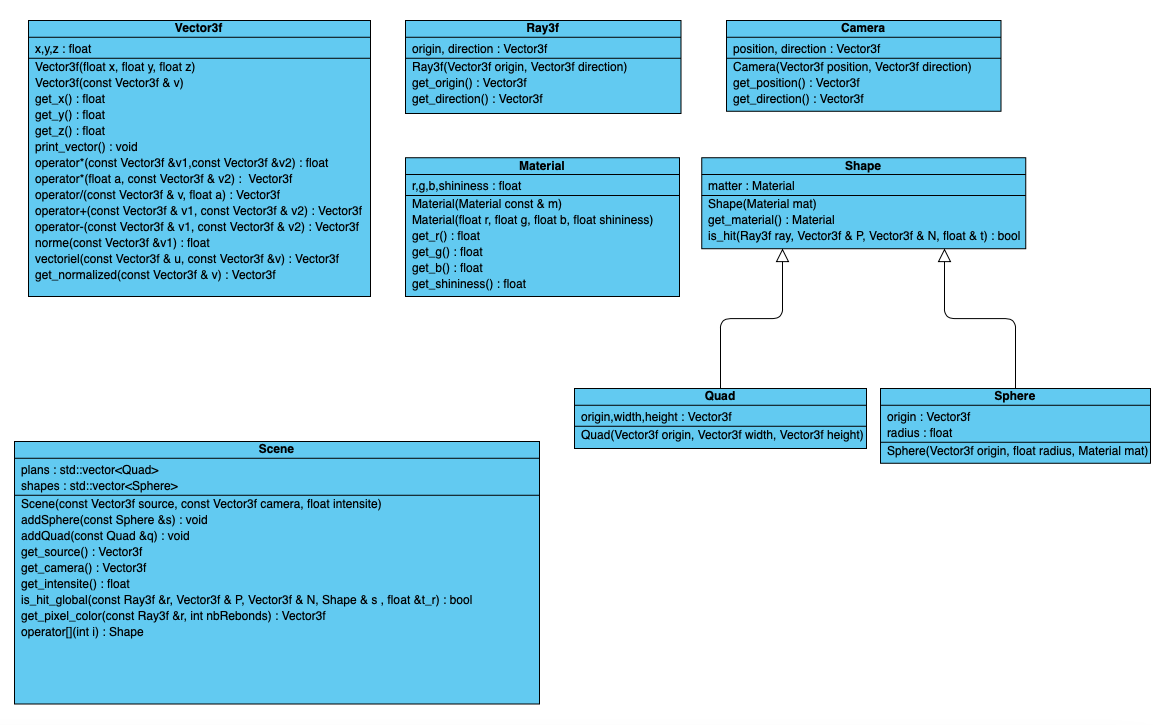
\includegraphics[scale=0.45]{rapport/UML.png}
    \caption{Diagramme de classes complet}
    \label{fig:my_label}
\end{figure}

\subsection{Libpng}
Pour initialiser et écrire les images nous avons, comme le sujet l'indique, utilisé \textit{libpng}. C'est une librairie externe au C++ et la comprendre et la maîtriser nous a pris du temps. Le traitement de l'image se fait grâce aux fonctions implémentées dans le fichier \textit{writing\_png.cpp}. Nous avons dans un premier temps codé une fonction permettant d'initialiser la structure de l'image en utilisant les structures données par \textit{libpng}. Nous écrivons les pixels de l'image dans trois listes R,G,B recevant des nombres flottants entre $0$ et $255$ et nous les assemblons et écrivons l'image avec notre dernière fonction qui écrit l'image puis libère l'espace occupé par les structure initialisées avec \textit{libpng}.

\subsection{Notre premier Ray Tracer}
Après avoir implémenté les classes \textit{Vector3f}, \textit{Ray3f} et \textit{Camera}, nous avons implémenté l'algorithme décrit dans la section 2.2 pour visualiser un disque blanc sur fond noir, sans nuance de couleur.
Nous n'avons pas rencontré de difficulté majeur et le résultat obtenu est re
présenté sur la figure 2.

\begin{figure}
    \centering
    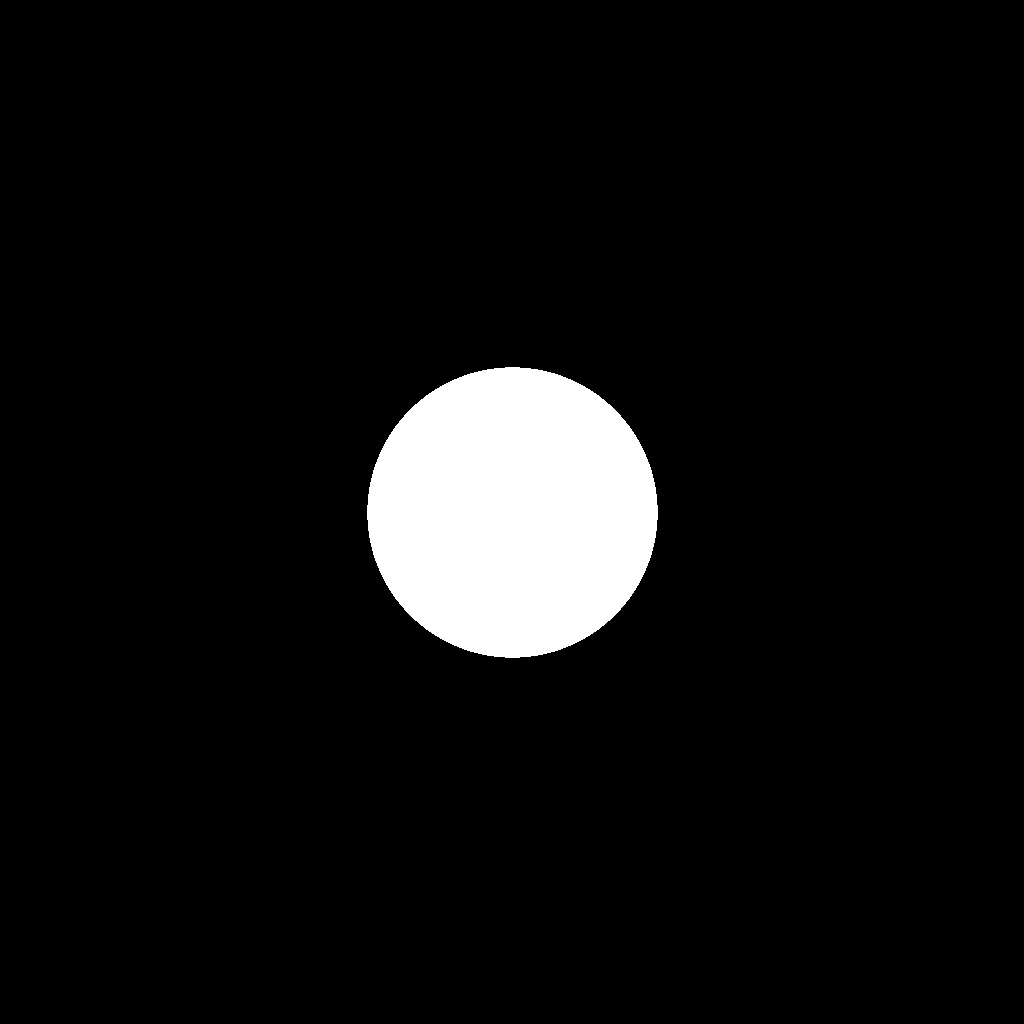
\includegraphics[scale=0.2]{rapport/result.png}
    \caption{Premier Ray Tracer}
    \label{fig:my_label}
\end{figure}

\subsection{Ajout d'une lumière}
L'étape suivant consistait en l'ajout d'une lumière au dessus de la sphère. Pour chaque pixel parcouru, nous recalculons sa luminosité en fonction de sa position par rapport à la lumière. La couleur du pixel au point P est donnée par $I = \lambda\frac{<(S-P),\vec{N}>}{||S-P||^2}$ où $\lambda$ représente l'intensité de la lumière, $S$ le point de source de la lumière, $P$ le point observé et $\vec{N}$ le vecteur unitaire normale au point observé. Nous complétons alors l'algorithme de la section \textbf{3.3} en écrivant des pixels d'une intensité $I$ calculé pour chaque point. On peut finalement constaté sur la Figure 3 que les points de la  sphère s'assombrissent en s'éloignant de la lumière placé en haut à gauche de l'image ici.

\begin{figure}
    \centering
    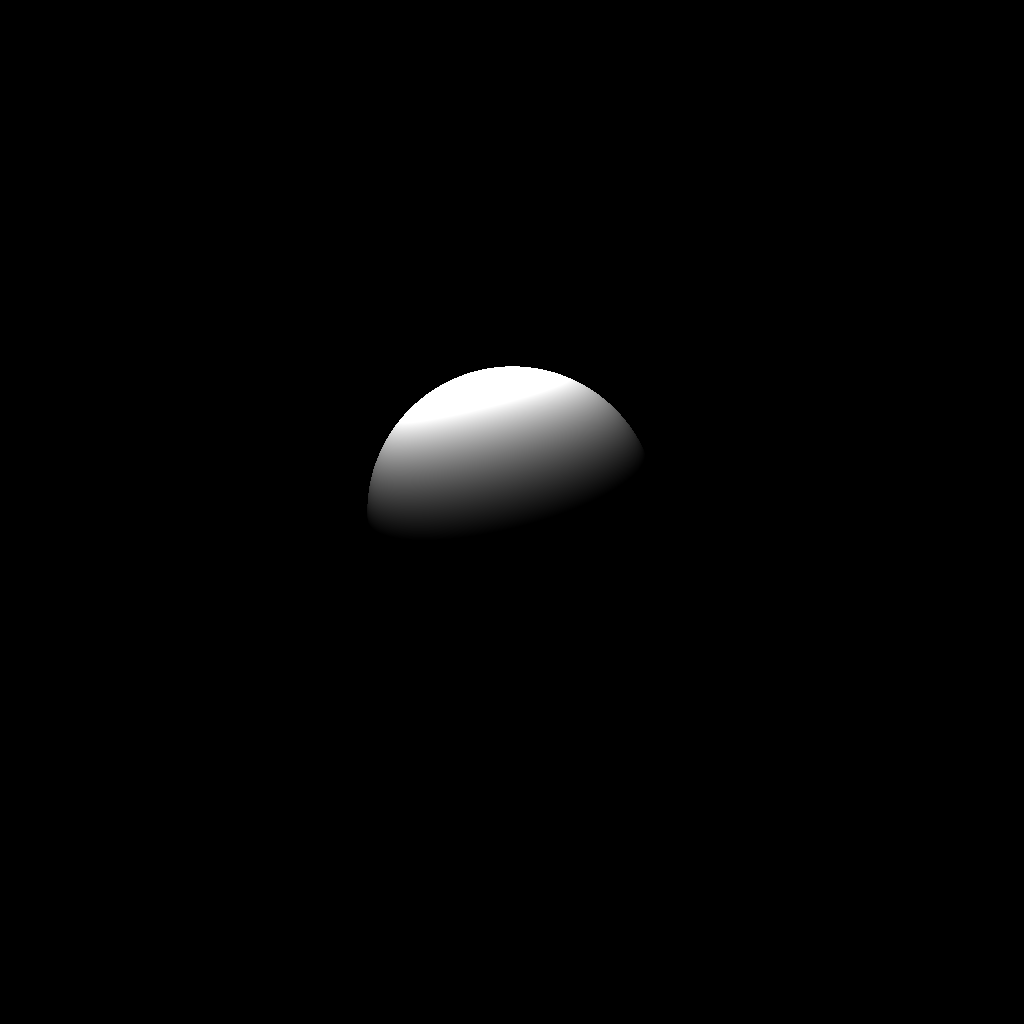
\includegraphics[scale=0.2]{rapport/result 2.png}
    \caption{Ajout d'une source lumineuse}
    \label{fig:my_label}
\end{figure}

\subsection{Les plans}
En parallèle de l'implémentation de la lumière, le deuxième membre du binôme a programmé une nouvelle classe héritant de la classe Shape : Quad. Cette classe représente les plans dans l'espace. Nous avons fait ici un mauvais choix qui nous empêchera d'ajouter des cubes au projet par la suite. En effet, l'origine du plan permet de situer le plan dans l'espace et les vecteurs \textit{width} et \textit{height} ont été interprété comme étant les vecteurs directeurs de la largeur et de la hauteur du plan. Nous nous sommes rendu compte de notre erreur en fin de projet ne nous laissant pas le temps de la corriger pour ajouter des cubes au projet (les plans étant infinis, ils ne permettent pas de former des cubes).
Pour déterminer s'il y a intersection entre un plan et le rayon, nous utilisons le fait que le point P observé est sur le plan si 
$$(P-P_0).\vec{n} = 0$$
Or $P = 0 + t*d_c$, donc il y a intersection si
$$(t*d_c-P_0).\vec{n} = 0$$
$$\iff t = \frac{(O_p - \vec{d_c}).\vec{n}}{\vec{n}*\vec{d_c}} \geq 0$$

Avec $\vec{n}$ le vecteur normal au plan résultant du produit vectoriel entre \textit{width} et \textit{height}, $O_p$ l'origine du plan.

Le calcul de la lumière pour le plan s'effectue de la même manière que pour la sphère avec la normale au point d'intersection entre le rayon tiré et le plan.

\subsection{La Scène}
Pour tout assembler, nous avons implémenté la Classe Scène contenant toutes les informations de la scène notamment les formes (plans et sphères),la position de la lumière et de la caméra et l'intensité de la lumière.
Lors de la compilation nous avons rencontré une erreur que nous n'avons pas su résoudre. En effet, la classe scène devait normalement contenir une liste de \textit{Shape}, mais lors du parcours de cette liste l'appel à la méthode \textit{is\_hit} entraîne une erreur de compilation et nous pensons que cela est dû à un problème d'implémentation de l'héritage des méthodes \textit{is\_hit} de \textit{Quad} et \textit{Sphere}

Nous avons alors décidé de séparer les formes en deux listes : les sphères et les plans. Pour gérer les intersections entre les rayons et les formes de la scène, il faut prendre en compte la distance entre la caméra et les points d'intersection dans le cas où des formes seraient alignés. Cela nous a un peu ralentit mais nous avons finalement réussi à gérer cela et nous pouvons constater le résultat obtenue sur la Figure 4.

\begin{figure}
    \centering
    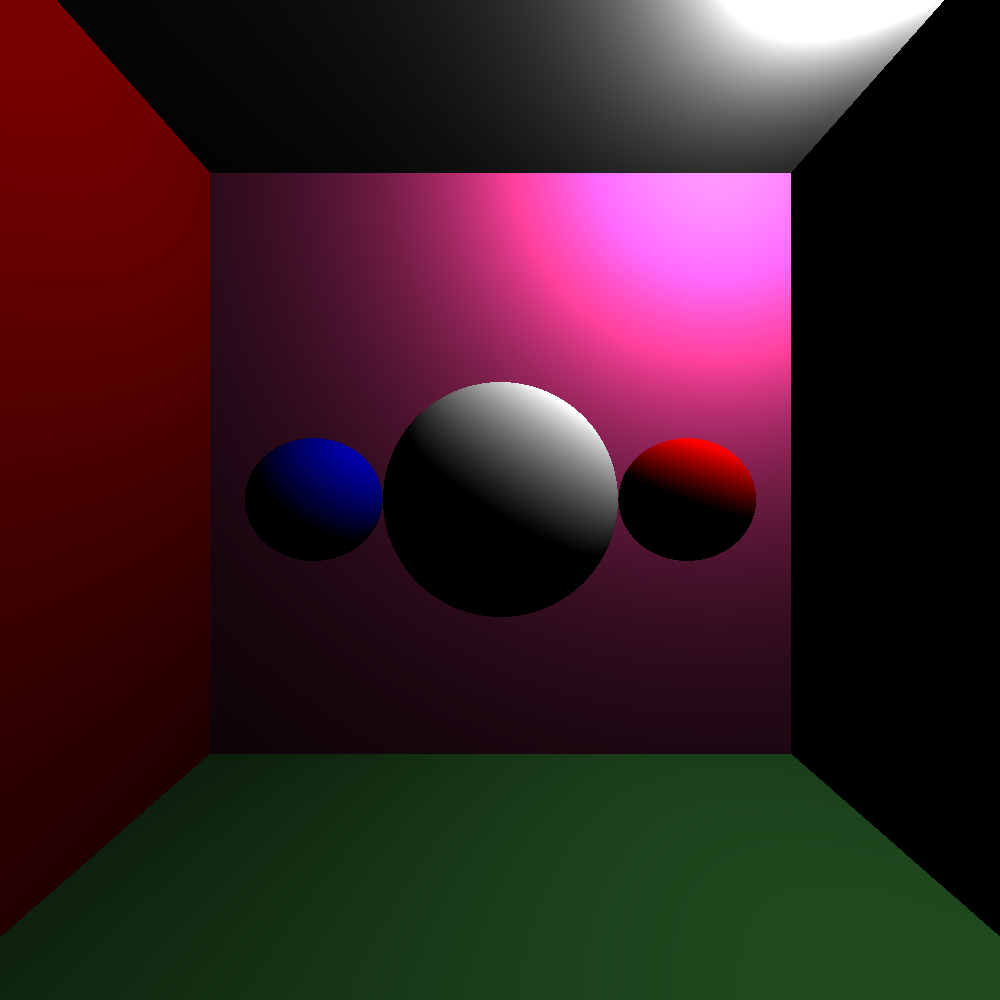
\includegraphics[scale=0.2]{rapport/result 3.png}
    \caption{Visualisation d'une scène contenant plusieurs formes}
    \label{fig:my_label}
\end{figure}

\subsection{Ajout des ombres}
Nous avons géré l'intensité de la lumière en fonction de la distance à la source mais il faut maintenant ajouter l'ombrage. Le principe n'est pas si compliqué : au point P observé, nous tirons un rayon en direction de la lumière et nous regardons s'il y a intersection avec une forme entre le point de tir et la source. Si tel est le cas, le pixel sera noir. Cependant nous avons rencontré un problème que nous avons tardé à résoudre.

\begin{figure}
    \centering
    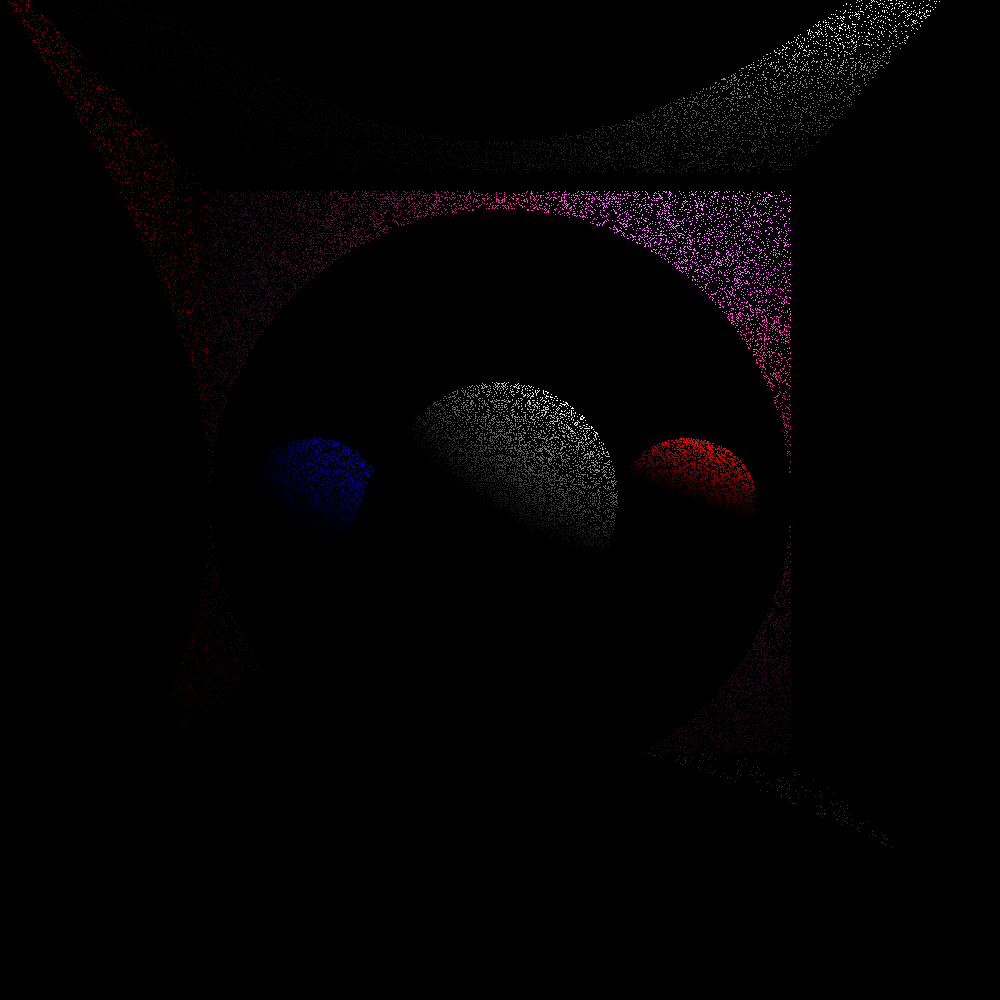
\includegraphics[scale=0.2]{rapport/result 4.png}
    \caption{Ombrage avant correction du bug}
    \label{fig:my_label}
\end{figure}

Sur la figure 5 nous voyons que le rendu n'est pas celui attendu car nous voyons de nombreuses tâches noirs ici et là. Après un long moment de débugague, nous nous sommes rendu compte que cela était dû à une imprécision numérique de l'ordinateur dans les calculs d'intersection. Pour les points noirs non souhaités, l'ordinateur détectait une intersection avec eux mêmes entraînant la génération d'une ombre non souhaitée. Pour corriger cela, il suffit de décoller un peut le point observé de la sphère en ajoutant au point le vecteur normal multiplié par $\epsilon = 0,1$. Le résultat obtenu sur la figure 6 est beaucoup plus satisfaisant.

\begin{figure}
    \centering
    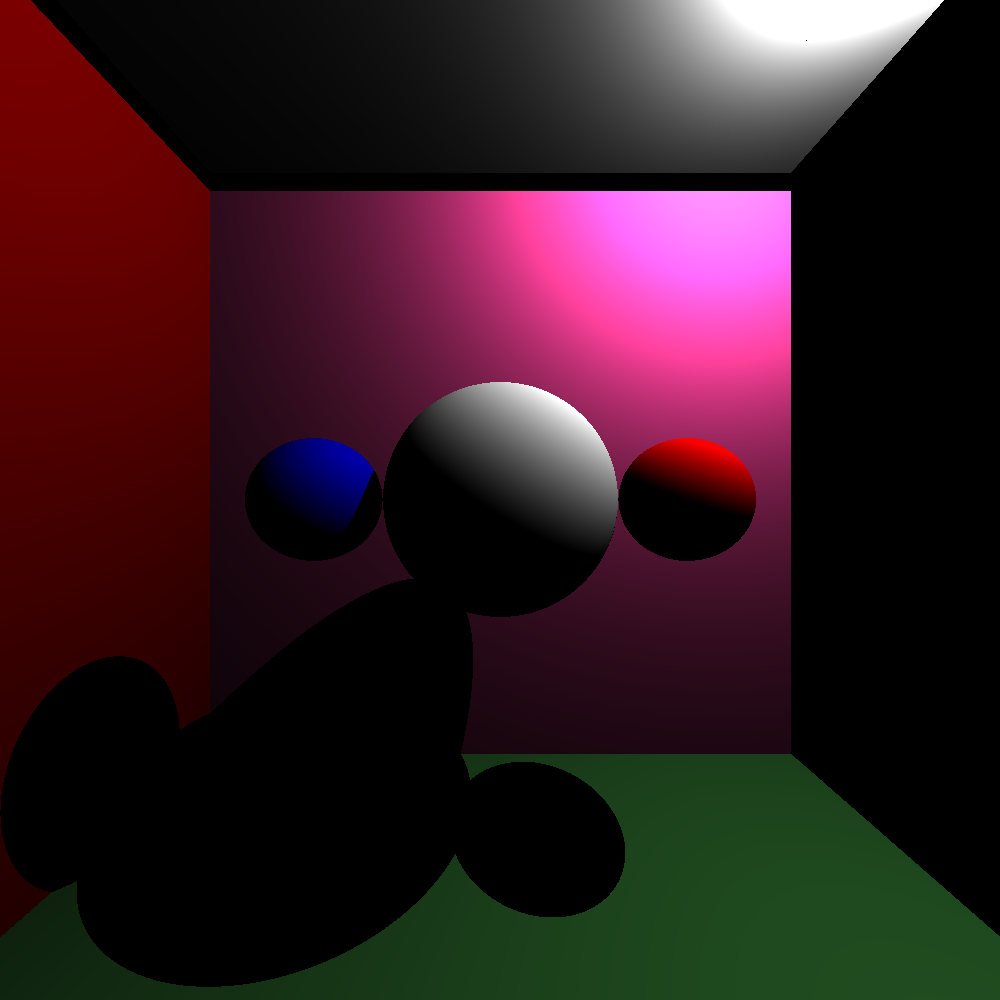
\includegraphics[scale=0.2]{rapport/result 5.png}
    \caption{Ombrage après correction du bug}
    \label{fig:my_label}
\end{figure}

\subsection{Réflexion}
Pour terminer le projet, nous avons ajouté la réflexion aux matériaux dont \textit{shininess} est supérieur à 0. Nous avons eu beaucoup de mal à réaliser cette partie car nous n'avions pas pensé à programmer une fonction récursive au début. Nous tentions de parcourir les rayons réfléchis mais se fût sans résultat. C'est seulement après réflexion que nous avons pensé à une fonction récursive. La méthode \textit{get\_pixel\_color} de la classe Scene est récursive et elle gère en plus de tout ce qui a été décrit avant la réflexion. Si le rayon courant touche une forme brillante, alors il est réfléchi et on rappel la fonction récursivement jusqu'à ce que le rayon incident touche une forme non brillante ou ne touche rien. Dans le cas où deux formes brillantes se feraient face, il y aurait un nombre infini de rayon réfléchis et donc un nombre infini de récursions. Pour éviter cela, la fonction prend en paramètre le nombre de rebonds maximum et la récursion s'arrête lorsque le nombre de récursion atteint cette limite.

Enfin, $shininess$ prend des nombres flottants quelconques. Si ce paramètre est inférieur ou égale à 0, alors il n'y a pas de réflexion et la forme est diffuse, si il est entre 0 et 1 alors la forme est plus ou moins brillante, si il est supérieur à 1 alors c'est un miroir. Observons le résultat sur les figures 7 et 8

\begin{figure}[!tbp]
  \centering
  \begin{minipage}[b]{0.4\textwidth}
    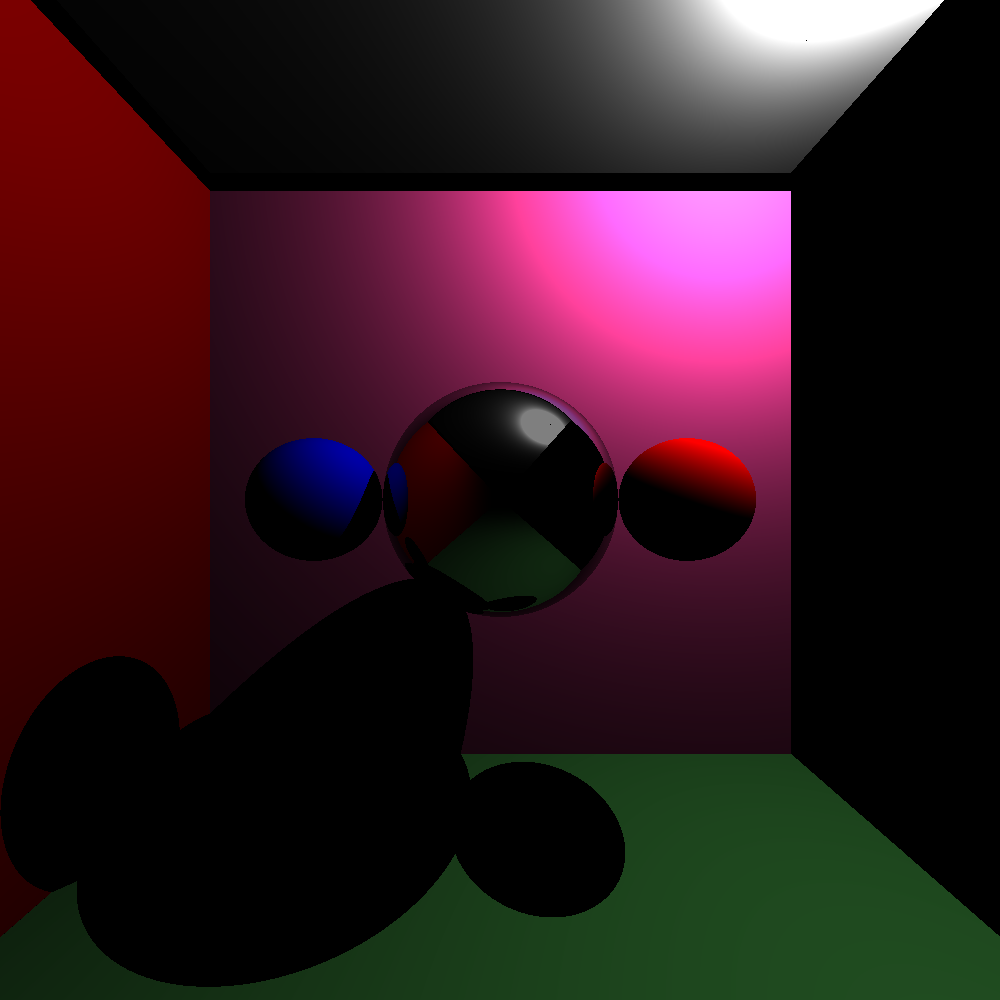
\includegraphics[width=\textwidth]{rapport/result 7.png}
    \caption{Scène \textit{shininess} faible}
  \end{minipage}
  \hfill
  \begin{minipage}[b]{0.4\textwidth}
    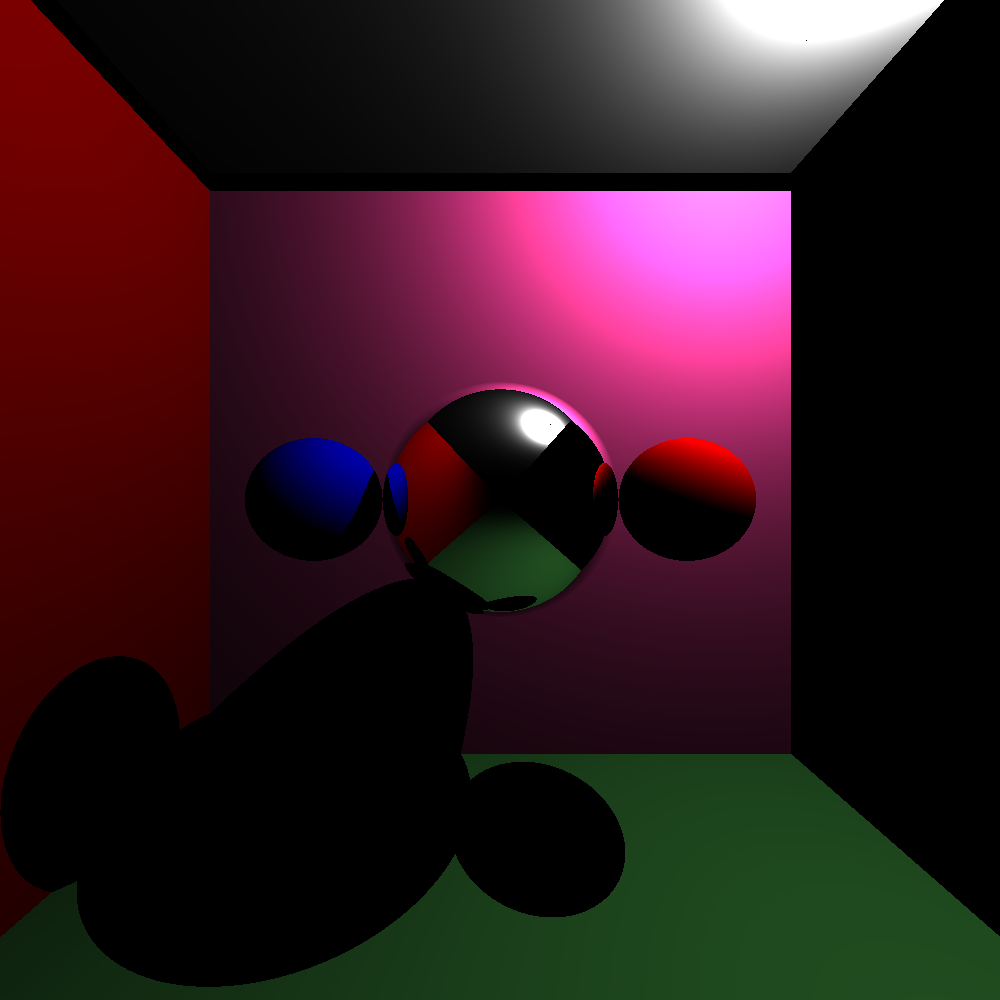
\includegraphics[width=\textwidth]{rapport/result 8.png}
    \caption{Scène avec \textit{shininess} élevée}
  \end{minipage}
\end{figure}

\section{Conclusion}
Nous sommes ravi du résultat obtenue avec notre ray tracer. Nous avons aimé réaliser ce projet en équipe d'autant plus que nous avons trouvé le sujet intéressant. Nous sommes cependant déçu de notre erreur nous empêchant par manque de temps d'implémenter les cubes. Cependant, une fois la Classe cube implémenté, il serait facile de l'ajouter à la scène car la réflexion ou l'ombrage fonctionnerait parfaitement dans notre environnement actuel.

Il est envisageable pour nous de poursuivre le ray tracer comme projet personnel pour y ajouter de nouvelles formes ou caractéristiques physiques comme les triangles pour réaliser des figures plus complexes, la diffraction en milieux transparents... Enfin une idée intéressante serait de créer des animations à l'aide de notre ray tracer en générant un grand nombre d'image mis bout-à-bout.

\section{Manuel d'utilisation}

Pour compiler le projet, il faut se rendre dans le dossier source avec un terminal et exécuter la commande :

\textbf{g++ material.cpp shape.cpp sphere.cpp vector3f.cpp ray3f.cpp main.cpp writing\_png.cpp quad.cpp utils.cpp scene.cpp -lpng -lz -o ray-tracer.o}

Et pour exécuter le projet : \textbf{./ray-tracer.o}

Pour modifier la scène, il faut ajouter ou modifier des formes dans la fonction main du fichier main.cpp.

\end{document} 